\section*{6. \"Ubung (Abgabe: 09.06.2010, 8.30 Uhr, schriftlich)}

\subsection*{1. Diskutieren Sie die komplexwertige Gabor-Transformation und ihre Fourier-Transformierte. Welchen Bezug sehen Sie zu der Klasse der Hermitischen Funktionen?}

\subsection*{2. Gegeben sei die zweidimensionale isotrope Gauss-Funktion: $Gauss_{\sigma}(x,y)$}
\subsubsection*{Berechnen Sie die Ableitung dieser Funktion nach $\sigma$, sowie die zweite Ableitung der Funktion nach x und die zweite Ableitung nach y.}
\subsubsection*{Wie stehen diese Ableitungen in Beziehung? Beachte: Die Summe der zweiten Ableitungen nach x undy wird als \emph{Laplacian of Gaussion} bezeichnet und stellt einen \"ublichen Kantenoperator dar.}
Siehe auch Abb. \ref{fig:1Abl}, \ref{fig:2Abl}, \ref{fig:LoG}.

\begin{figure}[p] %  figure placement: here, top, bottom, or page
   \centering
   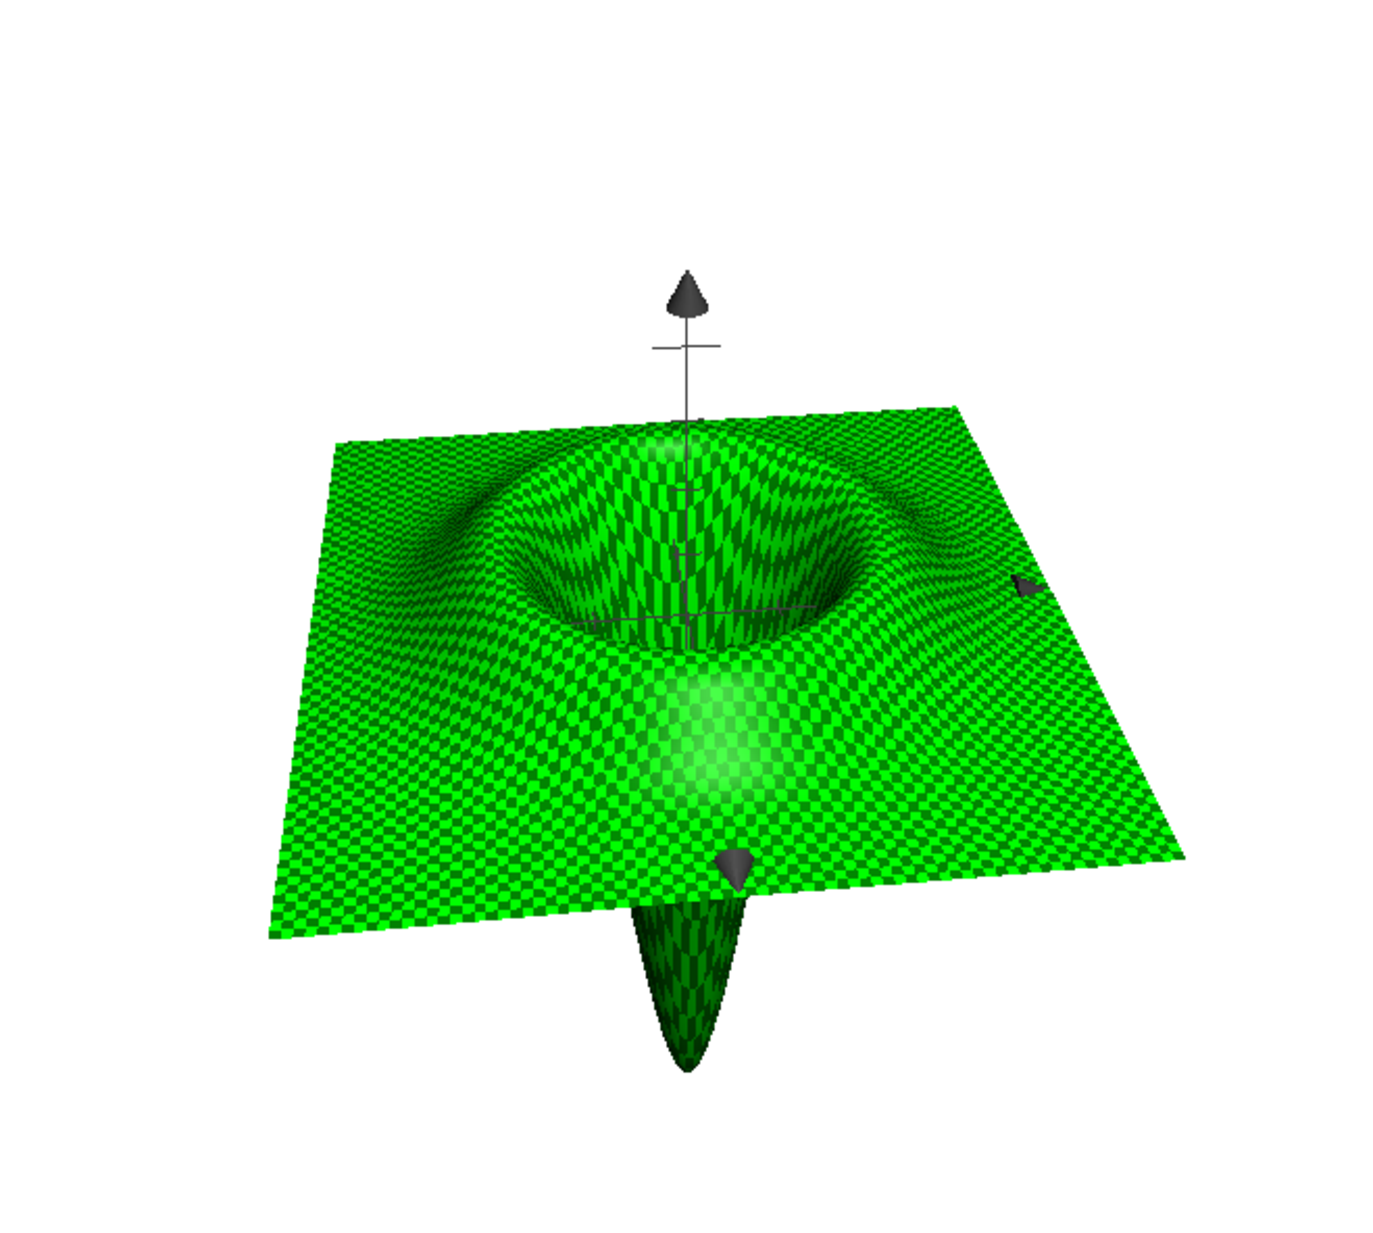
\includegraphics[width=0.4\textwidth]{Uebung6/1Abl_sigma.pdf} 
   \caption{$d^{2}/d\sigma$}
   \label{fig:1Abl}
\end{figure}

\begin{figure}[p] %  figure placement: here, top, bottom, or page
   \centering
   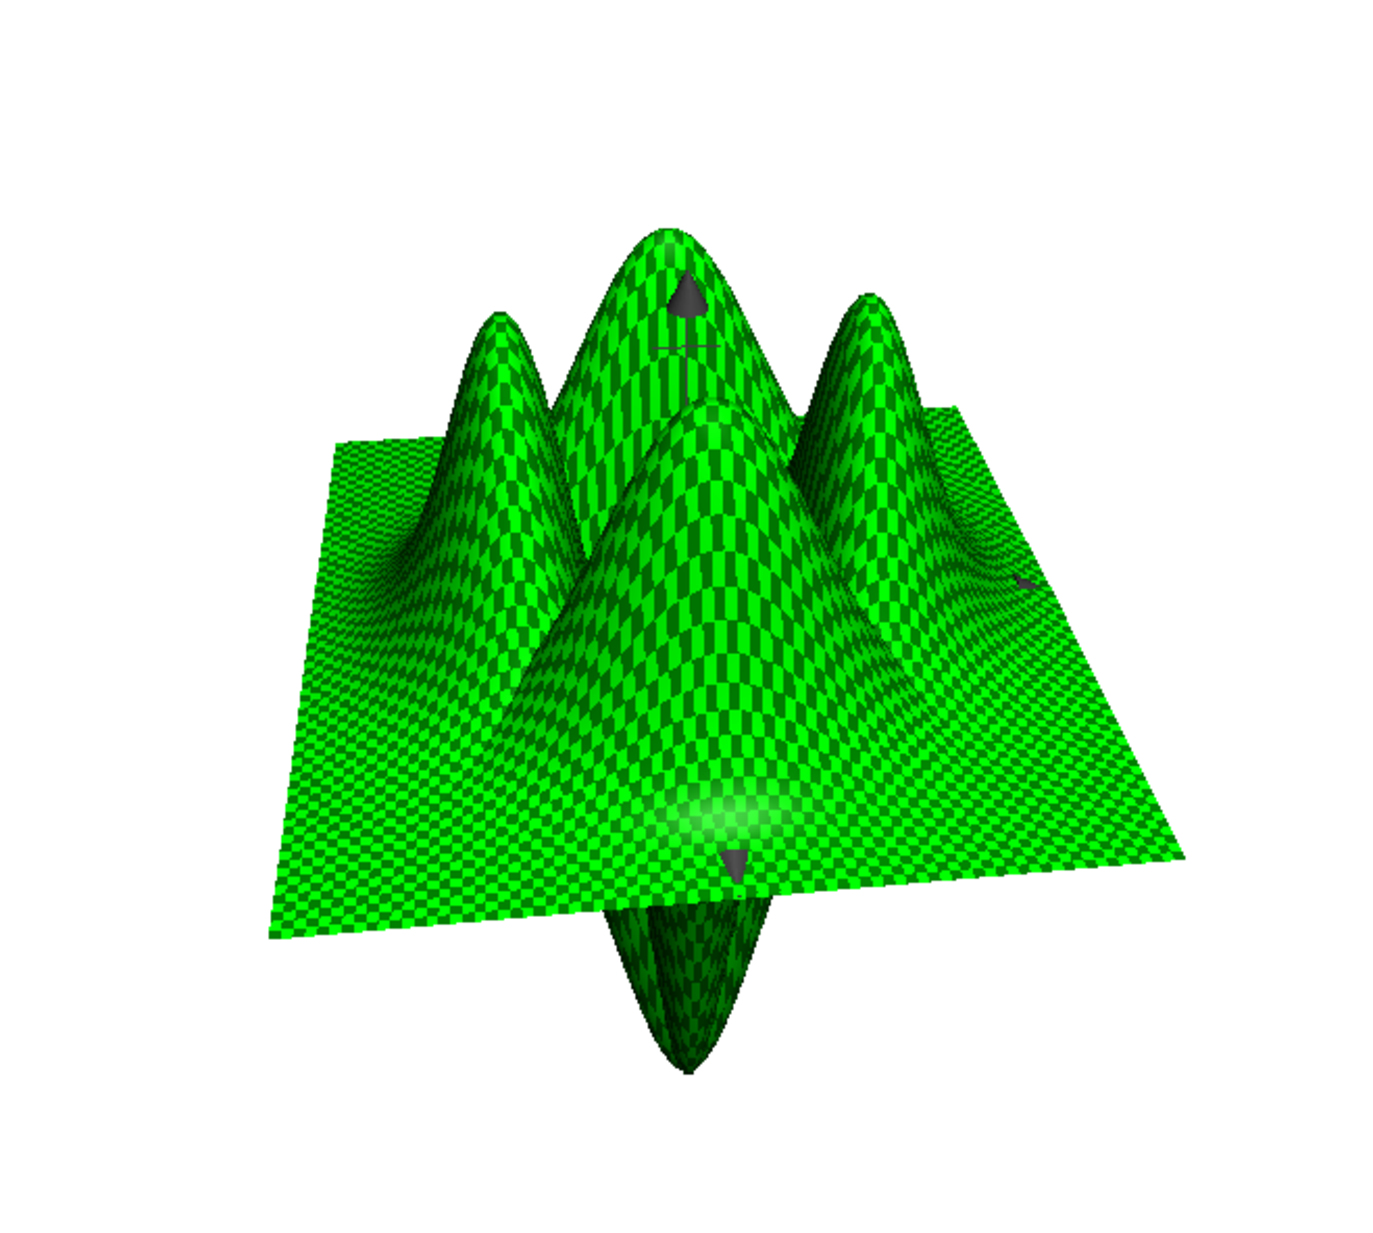
\includegraphics[width=0.4\textwidth]{Uebung6/2Abl_xy.pdf} 
   \caption{$d^{2}/dx^{2}$ und $d^{2}/dy^{2}$}
   \label{fig:2Abl}
\end{figure}

\begin{figure}[p] %  figure placement: here, top, bottom, or page
   \centering
   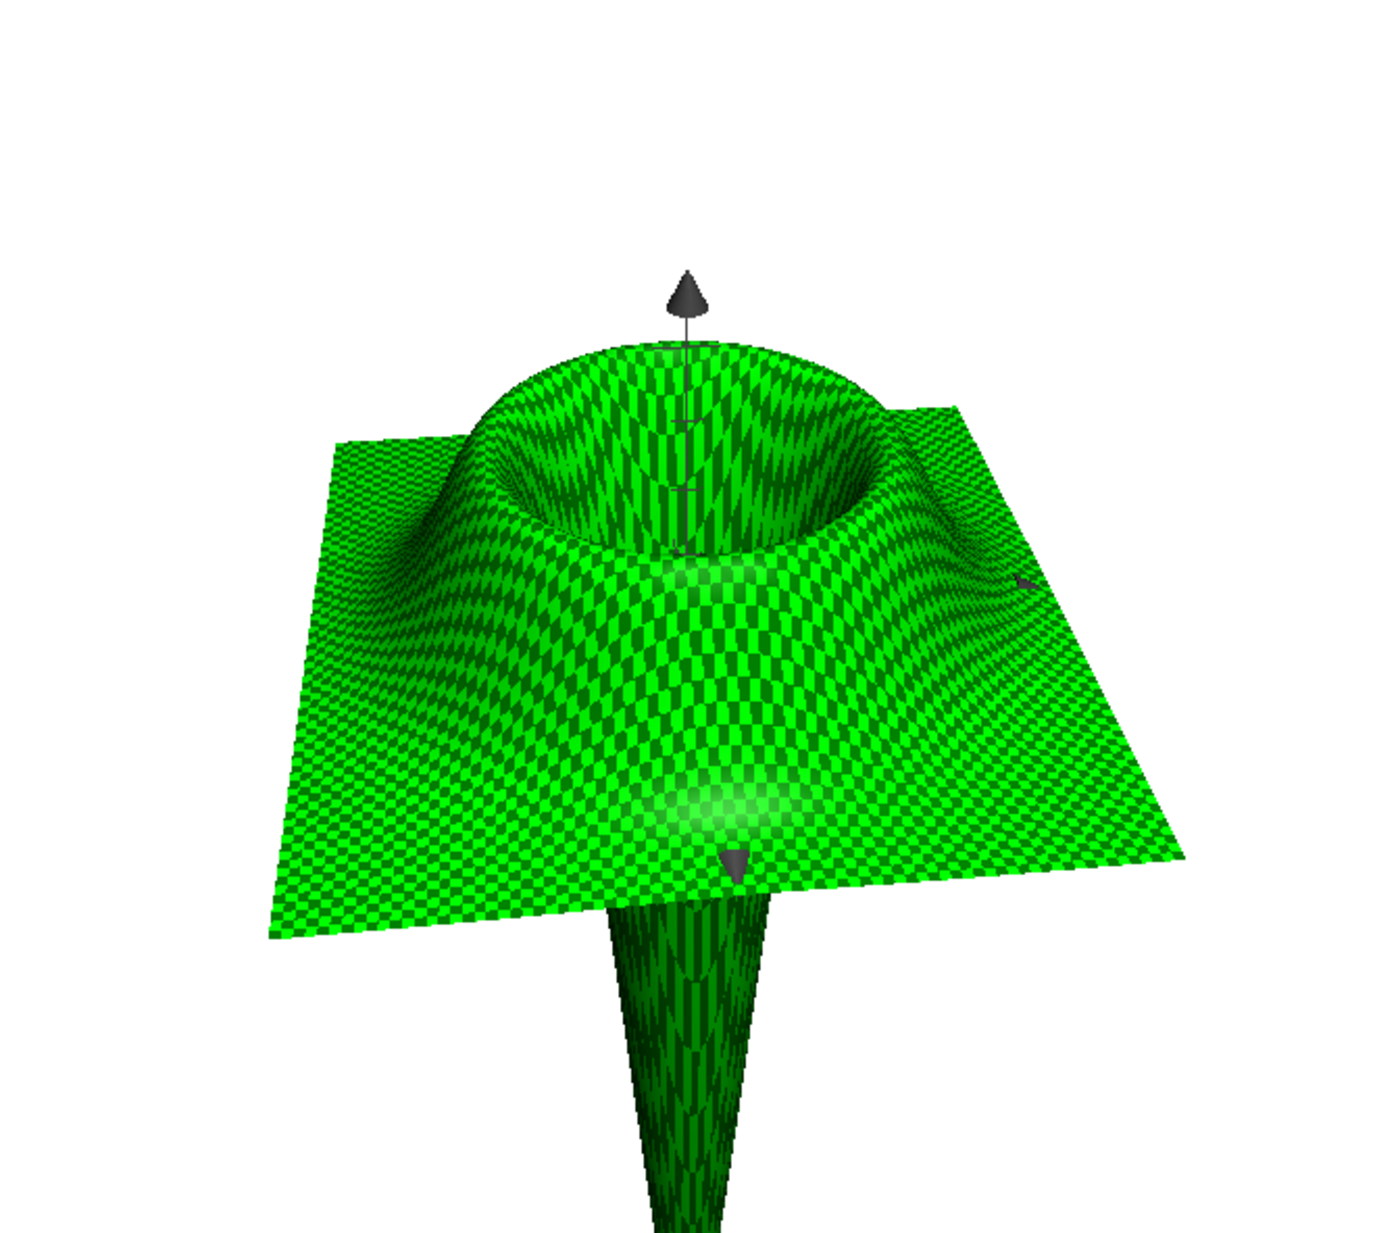
\includegraphics[width=0.4\textwidth]{Uebung6/LoG.pdf} 
   \caption{LoG}
   \label{fig:LoG}
\end{figure}

\subsubsection*{Wie kann man den \emph{Laplacian of Gaussion} in einem Gaussian Skalenraum effizient approximieren?}
